% Build from this directory: lualatex -interaction=nonstopmode -halt-on-error main.tex
\documentclass[12pt,a4paper]{article}
\usepackage{fontspec,polyglossia}
\setdefaultlanguage{ukrainian}
\setmainfont{NewCM10-Regular.otf}[BoldFont=NewCM10-Bold.otf,ItalicFont=NewCM10-Italic.otf,BoldItalicFont=NewCM10-BoldItalic.otf]
\setsansfont{Noto Sans}
\setmonofont{Noto Sans Mono}[Scale=0.82]
\usepackage{xurl}
\usepackage{geometry,graphicx,booktabs,array,enumitem,caption,titlesec,xcolor,fvextra}
\geometry{left=2cm,right=2cm,top=2cm,bottom=2cm}
\setlength{\parindent}{1.25cm}
\setlength{\parskip}{4pt}
\linespread{1.08}
\setlength{\emergencystretch}{3em}
\titleformat{\section}{\normalfont\fontsize{14}{16}\selectfont\bfseries}{\thesection}{0.6em}{}
\titleformat{\subsection}{\normalfont\fontsize{12}{14}\selectfont\bfseries}{\thesubsection}{0.6em}{}
\captionsetup{hypcap=false,font=small,labelfont=bf,labelsep=endash}
\DefineVerbatimEnvironment{code}{Verbatim}{fontsize=\footnotesize,breaklines=true,breakanywhere=true,frame=single,framesep=2mm}
\usepackage[unicode,colorlinks=true,linkcolor=black,urlcolor=blue,pdfauthor={Давидчук Артем},pdftitle={Архітектура комп'ютерів. Частина 2. Лабораторна робота №3}]{hyperref}
\begin{document}
\pagenumbering{gobble}
\begin{titlepage}
\begin{center}
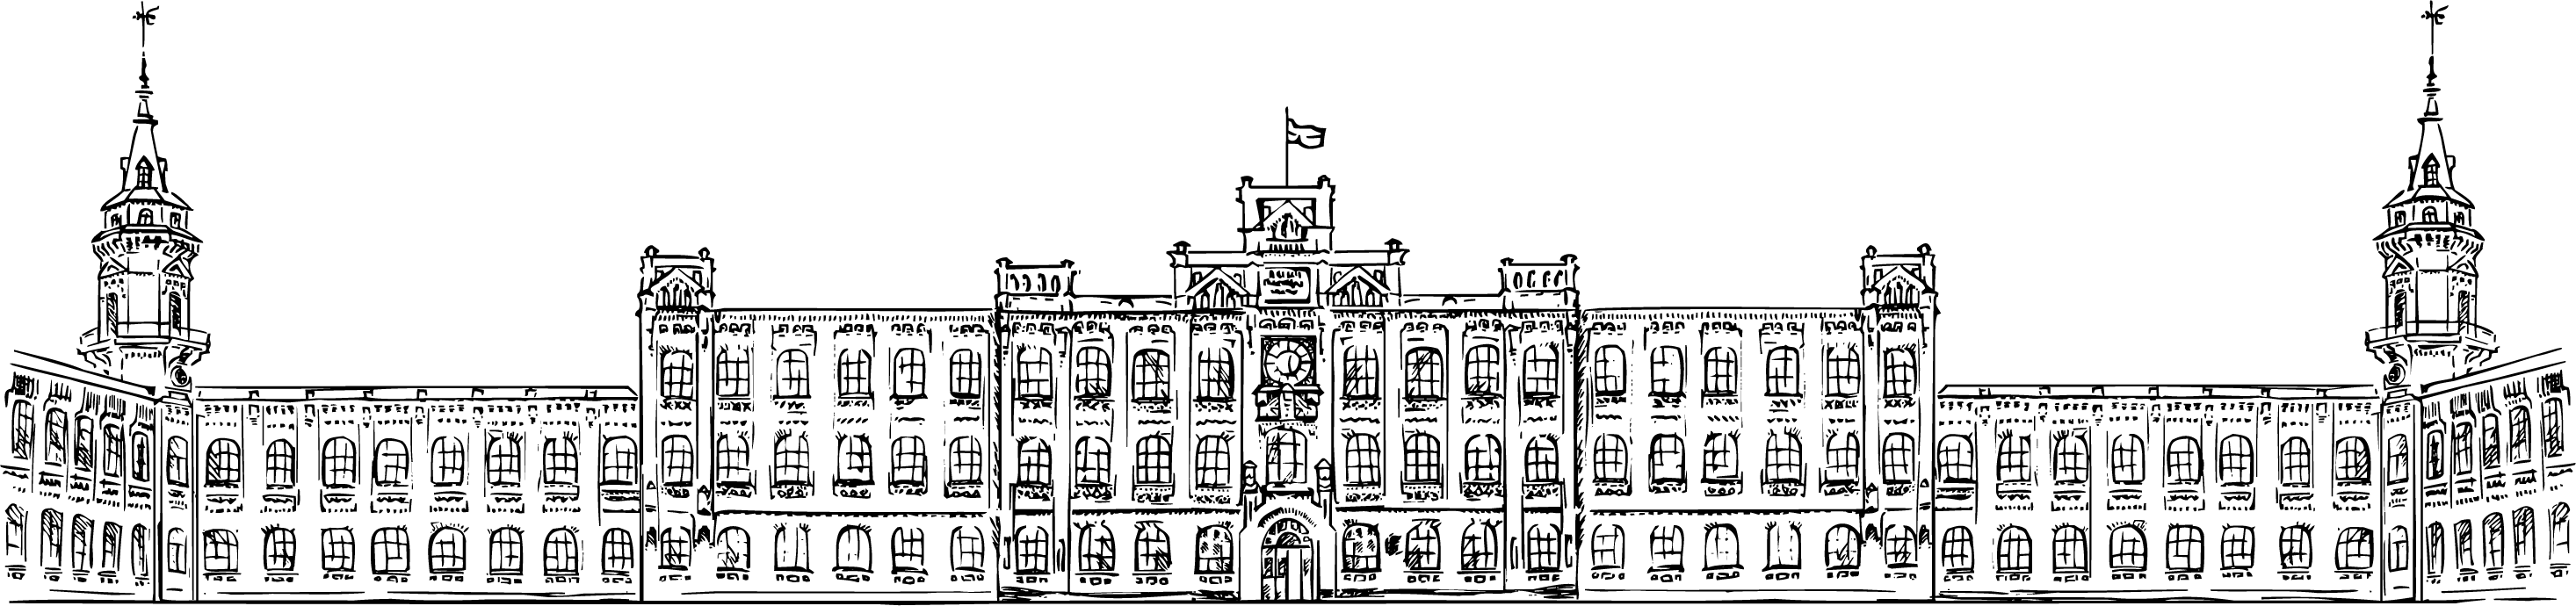
\includegraphics[width=0.7\textwidth]{../../../../../../templates/letterhead.png}\\[1em]
\large Національний технічний університет України\\
«Київський політехнічний інститут імені Ігоря Сікорського»\\[1em]
Факультет інформатики та обчислювальної техніки\\
Кафедра обчислювальної техніки
\end{center}
\vfill
\begin{center}
\textbf{\LARGE Архітектура комп'ютерів}\\[0.4em]
\textbf{\Large Частина 2. Процесори}\\[2em]
\textbf{\Large Лабораторна робота №3}\\[0.7em]
\parbox{0.9\textwidth}{\centering «Розвертання програмного забезпечення.\\Запуск Linux для ARM у середовищі QEMU»}
\end{center}
\vfill
\begin{flushright}
Виконав: студент групи ІО-41\\
\textit{Давидчук Артем}
\\[1em]Перевірив: \textit{Каплунов А.~В.}
\end{flushright}
\vfill
\begin{center}Київ --- 2026\end{center}
\end{titlepage}
\pagenumbering{arabic}
\section{Мета та завдання роботи}
Підготувати середовище кроскомпіляції для ARM, зібрати завантажувач U-Boot,
ядро Linux і BusyBox, сформувати мінімальну кореневу файлову систему та
перевірити її роботу в програмному емуляторі QEMU.

Виконано частини 1--3.1 інструкції \textit{BeagleBone Black: Platform Bring Up with Upstream Components}.
Пункти 1.3 і 1.4, що стосуються фізичного підключення плати, виключено
відповідно до завдання. Прошивання SD-карти та eMMC не виконувалось.
\section{Середовище та інструменти}
\begin{center}
\begin{tabular}{p{0.38\textwidth}p{0.53\textwidth}}
\toprule
\textbf{Компонент} & \textbf{Використане середовище}\\
\midrule
Основна система & Arch Linux, x86\_64\\
Кроскомпілятори & GNU Arm Toolchain 8.3-2019.03\\
Завантажувач & U-Boot v2019.07\\
Ядро гостьової системи & Linux 4.19.325, ARMv7\\
Користувацьке середовище & BusyBox 1.31.1\\
Емульована платформа & QEMU, машина \texttt{virt}, 512 МіБ RAM\\
Робочий каталог & \path{~/bbb-lab}\\
\bottomrule
\end{tabular}
\end{center}
Залежності встановлено засобами Arch Linux. Інструменти ARM розпаковано в
каталог користувача; системний компілятор не замінювався. Для кешування
результатів компіляції використано \texttt{ccache} з лімітом 5 ГіБ.
\begin{code}
sudo pacman -Syu --needed base-devel git curl wget \
  ccache ncurses openssl bc cpio python dtc qemu-system-arm
export BBB_LAB="$HOME/bbb-lab"
export CCACHE_DIR="$BBB_LAB/ccache"
ccache -M 5G
\end{code}
\section{Короткі теоретичні відомості}
Кроскомпіляція дозволяє на комп'ютері x86\_64 отримати виконувані файли для
ARM. U-Boot забезпечує початкове завантаження на фізичній платі. Ядро Linux
керує процесами, пам'яттю та пристроями, а BusyBox надає оболонку і набір
базових утиліт в одному виконуваному файлі.

У цій роботі QEMU безпосередньо завантажує \texttt{zImage} та архів
\texttt{initramfs}. Машина \texttt{virt} є узагальненою ARM-платформою,
а не емуляцією BeagleBone Black. Її опис пристроїв формує QEMU, тому
\texttt{MLO}, \texttt{u-boot.img} та DTB плати не передаються команді запуску.
\newpage
\section{Збирання U-Boot та ядра Linux}
\subsection{Налаштування кроскомпілятора}
Для U-Boot і ядра використано bare-metal toolchain з префіксом
\texttt{arm-eabi-}. Змінні встановлювались у поточній оболонці:
\begin{code}
export PATH="$BBB_LAB/toolchains/gcc-arm-8.3-2019.03-x86_64-arm-eabi/bin:$PATH"
export CROSS_COMPILE="ccache arm-eabi-"
export ARCH=arm
\end{code}
\subsection{Завантажувач U-Boot}
Вихідний код отримано з репозиторію U-Boot для версії \texttt{v2019.07}.
Конфігурація відповідає BeagleBone Black:
\begin{code}
cd "$BBB_LAB/repos/u-boot"
make am335x_boneblack_defconfig
make -j4
\end{code}
Для сумісності старого DTC із сучасним компілятором основної системи з
\path{scripts/dtc/dtc-lexer.l} вилучено повторне оголошення
\texttt{YYLTYPE yylloc;}. Це усуває помилку компонування
\texttt{multiple definition of yylloc}. Зміну збережено окремим патчем.
Системний GCC не понижувався. Отримано \texttt{MLO} (приблизно 108 КіБ)
і \texttt{u-boot.img} (приблизно 513 КіБ).
\subsection{Ядро Linux}
Використано стабільну гілку \texttt{linux-4.19.y}. Базову конфігурацію
\texttt{multi\_v7\_defconfig} доповнено фрагментом \texttt{bbb.cfg} з
підтримкою USB, USB HID, послідовних USB-адаптерів, мережевого мосту та
накладань Device Tree за методичкою.
\begin{code}
cd "$BBB_LAB/repos/linux-stable"
./scripts/kconfig/merge_config.sh \
  arch/arm/configs/multi_v7_defconfig fragments/bbb.cfg
make -j4 zImage modules am335x-boneblack.dtb
\end{code}
Отримано образ \path{arch/arm/boot/zImage} розміром приблизно 8,6 МіБ,
файл \path{arch/arm/boot/dts/am335x-boneblack.dtb} розміром приблизно
35 КіБ та модулі ядра версії \texttt{4.19.325}.

Після кожного етапу перевірявся результат команди. Вивід збирання
збережено в логах. Повторна перевірка наявних образів та їхніх точних
розмірів наведена у файлі \path{evidence/artifacts.txt}.
\newpage
\section{BusyBox і коренева файлова система}
Для BusyBox використано Linux toolchain, який містить бібліотеки glibc,
та гілку \texttt{1\_31\_stable}:
\begin{code}
export PATH="$BBB_LAB/toolchains/gcc-arm-8.3-2019.03-x86_64-arm-linux-gnueabihf/bin:$PATH"
export CROSS_COMPILE="ccache arm-linux-gnueabihf-"
export ARCH=arm
cd "$BBB_LAB/repos/busybox"
make defconfig
make -j4
make CONFIG_PREFIX="$BBB_LAB/repos/busybox/_install" install
\end{code}
BusyBox зібрано з динамічним компонуванням. Перевірка \texttt{file}
показала 32-бітний ELF для ARM EABI5 з інтерпретатором
\path{/lib/ld-linux-armhf.so.3}. Необхідні спільні бібліотеки скопійовано
з \texttt{sysroot} toolchain до \path{_install/lib}.

У \texttt{\_install} створено каталоги \texttt{boot}, \texttt{dev},
\path{etc/init.d}, \texttt{lib}, \texttt{proc}, \texttt{root},
\path{sys/kernel/debug} та \texttt{tmp}. Посилання
\texttt{/init -> bin/busybox} задає початковий процес системи.
\subsection{Стартовий скрипт}
Файл \path{_install/etc/init.d/rcS} зроблено виконуваним:
\begin{code}
#!/bin/sh
mount -t sysfs none /sys
mount -t proc none /proc
mount -t debugfs none /sys/kernel/debug
echo /sbin/mdev > /proc/sys/kernel/hotplug
mdev -s
\end{code}
До \path{/boot} скопійовано ядро, DTB, \texttt{System.map} і
конфігурацію ядра. Модулі встановлено тільки в навчальну файлову систему:
\begin{code}
make -C "$BBB_LAB/repos/linux-stable" \
  INSTALL_MOD_PATH="$BBB_LAB/repos/busybox/_install" modules_install
\end{code}
У \path{/etc} підготовлено файли \texttt{passwd}, \texttt{group},
\texttt{shadow}, \texttt{resolv.conf} і правило \texttt{mdev.conf} для
завантаження модулів за подіями пристроїв.
\subsection{Створення initramfs}
\begin{code}
cd "$BBB_LAB/repos/busybox/_install"
find . -print0 | cpio --null -o --format=newc --owner=0:0 \
  | gzip > ../rootfs.cpio.gz
\end{code}
В архіві файли мають власника \texttt{root}; їхні власники в основній
системі не змінюються. Розмір стисненого архіву становить приблизно 25 МіБ.
\newpage
\section{Запуск у QEMU}
Ядро й архів файлової системи завантажено такою командою:
\begin{code}
cd "$BBB_LAB/repos/busybox"
qemu-system-arm \
  -machine virt -m 512 -nographic \
  -kernel _install/boot/zImage \
  -initrd rootfs.cpio.gz \
  -append "root=/dev/ram0 rw console=ttyAMA0,115200 mem=512M"
\end{code}
Параметр \texttt{-kernel} задає образ ядра, \texttt{-initrd} --- архів
кореневої файлової системи, \texttt{-m 512} --- обсяг оперативної пам'яті.
Параметри \texttt{-nographic} і \texttt{console=ttyAMA0,115200} спрямовують
консоль гостьової системи в термінал.

\begin{center}
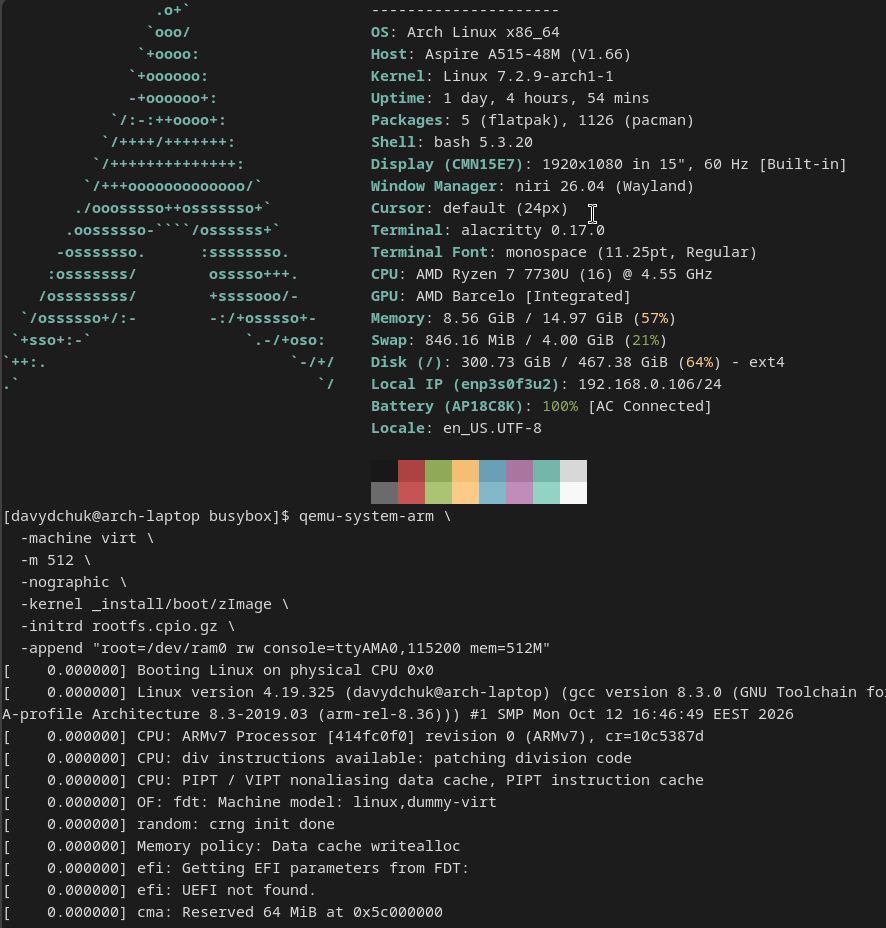
\includegraphics[width=0.76\textwidth]{../image1.png}
\captionof{figure}{Початковий запуск ядра ARM у QEMU, зафіксований 12.10.2026}
\end{center}
\newpage
\section{Перевірка працездатності}
Після завантаження та натискання Enter отримано командний рядок
\texttt{/ \#}. Виконано всі перевірки з пункту 3.1 методички:
\begin{code}
uname -a
ls -l
dmesg | grep init
busybox --help | head -15
poweroff
\end{code}
\begin{center}
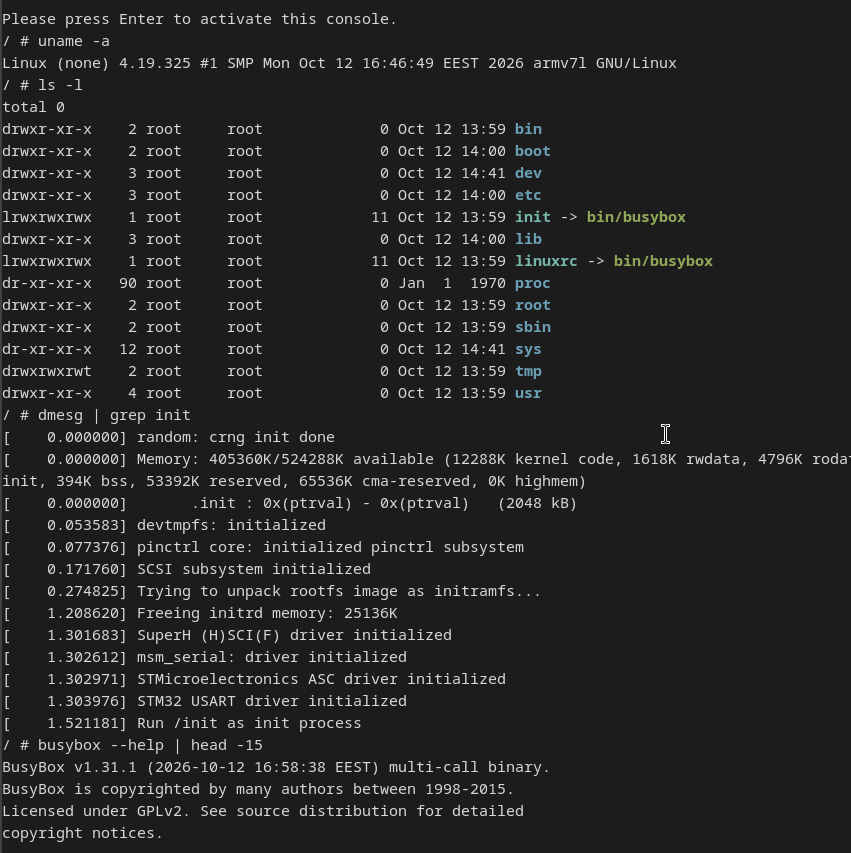
\includegraphics[width=0.83\textwidth]{../image2.png}
\captionof{figure}{Перевірка версії ядра, файлової системи та BusyBox}
\end{center}
\newpage
\section{Аналіз результатів}
Первинний запуск виконано 12.10.2026. Під час підготовки звіту 19.10.2026
збережені образи повторно запущено в QEMU без повторного збирання.
Перевірено також \texttt{cat /proc/cpuinfo} та \texttt{mount}.
Нижче наведено вибрані рядки фактичного виводу повторної перевірки:
\begin{code}
Linux (none) 4.19.325 #1 SMP Mon Oct 12 16:46:49 EEST 2026 armv7l GNU/Linux
BusyBox v1.31.1 (2026-10-12 16:58:38 EEST) multi-call binary.
model name      : ARMv7 Processor rev 0 (v7l)
CPU architecture: 7
rootfs on / type rootfs (rw)
none on /sys type sysfs (rw,relatime)
none on /proc type proc (rw,relatime)
none on /sys/kernel/debug type debugfs (rw,relatime)
\end{code}
Позначення \texttt{armv7l} підтверджує виконання ARM-ядра. Повідомлення
\texttt{Trying to unpack rootfs image as initramfs} та
\texttt{Run /init as init process} підтверджують розпакування файлової
системи та запуск початкового процесу. Вивід \texttt{mount} засвідчує
роботу стартового скрипту. Значення \texttt{(none)} означає, що ім'я
гостьової системи не було задано.

У журналі є попередження щодо PCI: \texttt{probe ... failed with error -16}.
Отже, успішна перевірка стосується запуску ядра, initramfs і консольного
середовища; працездатність усіх пристроїв або мережі не перевірялася.

Під час вимкнення мінімальна система повідомила про відсутність
\path{/etc/fstab} та неможливість відмонтувати корінь initramfs.
Після цього виконано \texttt{reboot: Power down}; процес QEMU завершився
з кодом 0. Повний вивід повторного запуску збережено в
\path{evidence/qemu-verification.txt}.
\section{Висновки}
Підготовлено середовище кроскомпіляції в Arch Linux та зібрано U-Boot,
ядро Linux 4.19.325 і BusyBox 1.31.1 для ARM. Сформовано мінімальну
кореневу файлову систему з бібліотеками, модулями ядра та стартовим скриптом.
Систему успішно запущено на віртуальній ARM-платформі QEMU з 512 МіБ RAM.

Перевірками підтверджено запуск \path{/init}, роботу оболонки,
базових утиліт, \texttt{procfs} і \texttt{sysfs}. Виконано обов'язкову
частину завдання до пункту 3.1 включно. Зібране ядро не встановлювалось
як ядро основної системи, фізична плата не використовувалась.
\section*{Використані матеріали}
\begin{enumerate}[leftmargin=*,nosep]
\item Sam Protsenko. \textit{BeagleBone Black: Platform Bring Up with Upstream Components}. Rev C3, 23 March 2020. Частини 1--3.1.
\item Журнал первинного запуску \texttt{output.txt} і скриншоти \texttt{image1.png}, \texttt{image2.png}.
\item Журнал повторної перевірки \path{evidence/qemu-verification.txt}, 19.10.2026.
\end{enumerate}
\end{document}
